%% Fiktivní kapitola s ukázkami sazby

\chapter{Návrh řešení}

V této kapitole je popsán návrh technického řešení uvedených problémů.

\section{Úvod}

Běh celé aplikace bude rozdělen do dvou částí.

\begin{itemize}
	\item Stahování a ukládání real-time dat o polohách vozidel do datového skladu, které budou doplněny o odhad zpoždění pro okamžité zveřejnění v uživatelské aplikaci.

	\item Modelování profilů jízd jednotlivých úseků. Tyto modely budou pak dále sloužit k odhadování zpoždění v budoucnu.  Výpočet modelů bude prováděn jednou za delší časový úsek (nejlépe jednou za den).
\end{itemize}

Protože obě části jsou na sobě závislé v iniciálním běhu bude prováděna první část sběru dat bez odhadu zpoždění, nebo pomocí již existujícího triviálního lineárního odhadu.

\bigbreak

Schéma návrhu celé aplikace a komunikační mapa jednotlivých komponent je ilusrtována na diagramu \ref{fig:design_diagram}.

\begin{figure}
	\centering
  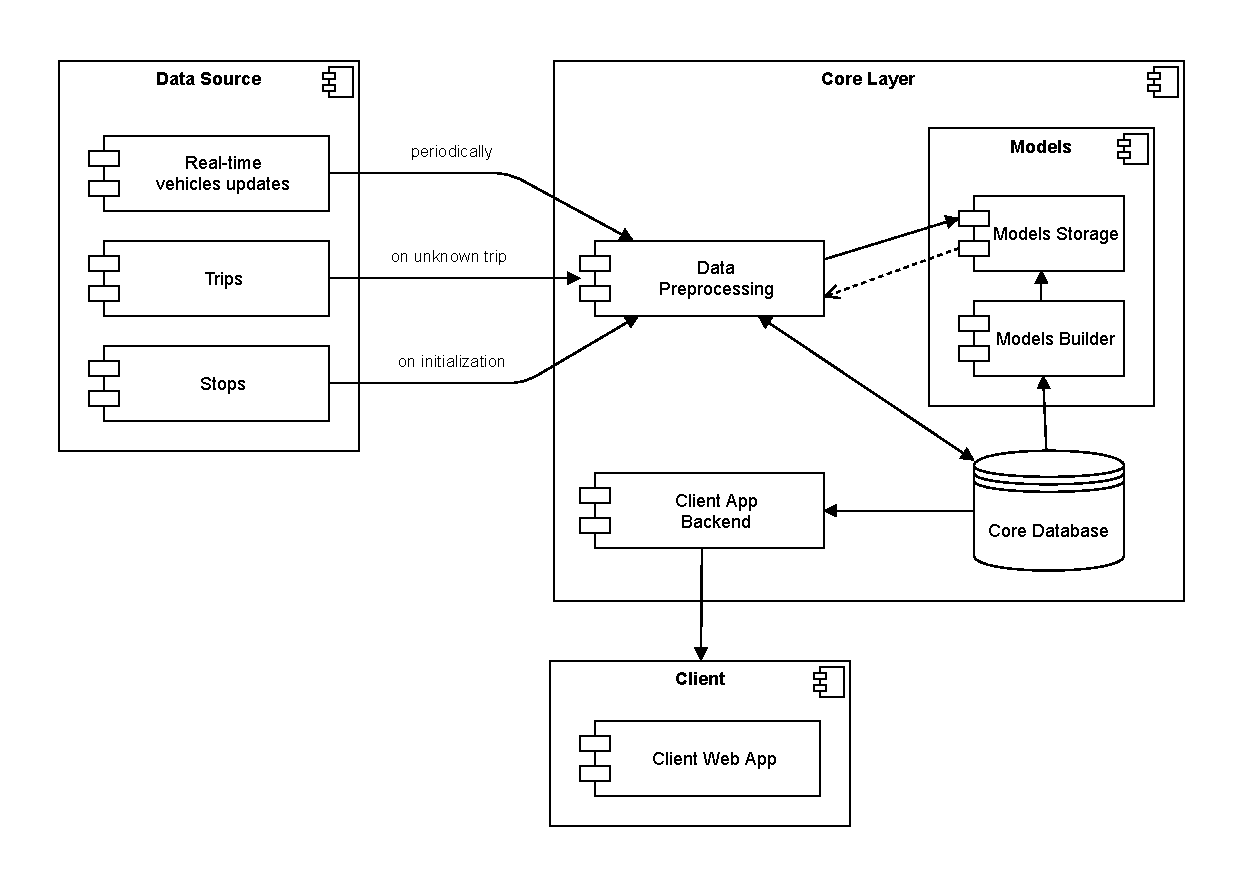
\includegraphics[width=\linewidth]{../img/design_diagram}
  \caption{UML diagram návrhu aplikace}
  \label{fig:design_diagram}
\end{figure}

\subsection{Funkční a kvalitativní požadavky}

Nejprve specifikujme požadavky systému, na kterém se pak bude zakládat
konkrétní návrh řešení jádra celé aplikace (bez backendu vizualizace).

\subsubsection{Funkční požadavky}

\begin{itemize}
	\item
Popsaný odhad změny zpoždění na trase mezi dvěma referenčními body je nutné počítat v co nejkratším čase tak, aby cestující byli dobře informování o stavu jejich spoje a mohli tyto informace využít např. při dobíhání spoje. A proto je potřeba zpracovávat data okamžitě po jejich vydání, spočítat odhad zpoždění a vystavit tato data veřejně. Vzhledem k tomu, že tato data velmi rychle zastarávají je nutné provádět tento proces co možná nejrychleji\footnote{Průměrná doba jízdy spoje mezi zastávkami je cca 5 min. Rozložení počtu úseků mezi zastávekami k délce jízdy mezi nimi je závislé a podobné rozložení vůči vzdálenosti ilustrované na grafu\ref{fig:stop_distances_result}.}.

\item

Data o polohách vozidel VHD v Datové platfomě jsou aktualizována nejpozději každých 20 sekund, více v kapitole \ref{chapter:analyza_zdroje}. Tedy pro minimalizaci rychlosti zastarávání dat a získání všech existujících vzorků dat o polohách je nutné data stahovat alesponˇ každých 20 sekund.

\item

Odhad zpoždění se bude provádět na základě historických dat z posledních vyšších jednotek dnů\footnote{Pro demonstrativní účely této práce jsou využívány historická data pouze ze 4 dnů (2 pracovní a 2 víkendové).}. Tím se sníží dopad mimořádné události na předpovědní model, která může na trase vzniknout. Zárovenˇ by však neměla být započítávána data starší několik týdnů, protože dopravní situace se mění v závislosti na ročním období nebo také pokud se na trase vyskytne delší omezení dopravy. Pak je požadováno, aby se takové omezení projevilo v modelu profilu jízdy co možná nejdříve. Navíc se bude rozlišovat mezi daty z pracovních dnů a nepracovních dnů, to protože samotné jízdní řády se mohou lišit\footnote{Ve dnech pacovního volna se v některých případech liší doba jízdy mezi mezastávkama pro stejnou dvojci zastávek. A to je porušení základního předpokladu z kapitoly \ref{section:zakladni_predpoklady} Základní předpoklady.} a také se do velké míry liší hustota dopravy, která ma velký vliv na profil jízdy. TODO do navrhy na zlepseni: Pro zpřesnění výsledků by bylo lepsi respektovat svatky, kazdy den v tydnu zvlast atp.

\item

Zpracování historických dat bude probíhat vždy po delší době, nejlépe jednou za den. To umožní provádět náročnější výpočty, které by za normálního provozu neúměrně přetížily systém. Navíc vzhledem k povaze cíle práce ani není žádoucí zpracování historických dat provádět častěji než jednou denně, protože se nepokoušíme okamžitě reagovat na změnu dopravní situace, ale modelovat profil jízdy vždy až pro celý den.

\item

Uložená historická data budou struktorovaná tak, aby nad nimi mohly být prováděny statistické výpočty minimálně o frekvencích jízd spojů, vzdálenostech tras a zpoždění spojů.
\end{itemize}

\subsubsection{Kvalitativní požadavky} \label{subsubsection:kvalitativni_pozadavky}

\begin{itemize}

	\item
	Řešení bude schopno při jedné aktualizaci zpracovat alesponˇ 1000\footnote{20. 2. 2020 mezi 7:00 a 7:10 bylo na trase přes 600 vozidel} vzorků poloh vozidel, kde 10 \% vzorků může být o dosut neznámých jízdách. V tomto případě je potřeba stáhnout jízdní řád konkrétní jízdy a její jízdní profil, což představuje navíc dotaz na Datovou platformu jakožto zdroje dat pro tuto práci.

	\item
	Vypočítané modely profilů jízd budou dávat odhad zpoždění lepší (až na vyjimku popsanou níže), než je lineární odhad. To znamená, že zpoždění vypočítaná pro každý přijatý vzorek polohy vozidla mezi dvěma referenčními body na trase bude mít menší rozptyl než lineární odhad zpoždění.

	\item
	V případě, že spočítaný odhad zpoždění vozidla by zastaral natolik rychle, že v okamžik zveřejnění by již nebyl platný, nedává smysl zpoždění odhadovat pokročilejší metodou.

\end{itemize}


\section{Zpracování vstupních dat} \label{section:zpracovani_vstupnich_dat}

Struktura uložení dat se zakládá na struktuře zdrojových dat popsaných v kapitole \ref{section:analyza_zdroje} Analýza zdroje dat.

\bigbreak

Na datové platformě jsou real-time data o vozidlech dostupná do historie řádově jednotek minut, což je naprosto nedostatečné pro jakékoliv pozdější využití v ránci této práce. Především pro počítání statistik a modelování profilů jízd nad daty je potřeba zřídit lokální databázi, která bude držet historická data tak, jak byla obdržena od zdroje. Navíc data jsou poskytována ve formátu \gls{json}, který svou povahou není zrovna úsporný co se do velikosti souboru týče. Proto je vhodné zvolit ukládání dat v jiném formátu.

\subsection{Databáze} \label{subsection:databaze}

Za tímto účelem tato práce využívá relační databázi obsluhovanou dotazovacím jazykem \gls{sql}. Struktura databáze je vyobrazena na EER diagramu \ref{obr:EER}\footnote{SQL dotazy na sestavení celé databaze jsou definovány v příloze database.sql. Pro testovací, debugovací a demonstrační účely slouží navíc i jiné databáze, které jsou struktorou totožné jako produkční databáze.}. Tato databáze se skládá z 5 tabulek. Jsou jimi:


\begin{figure}[p]\centering
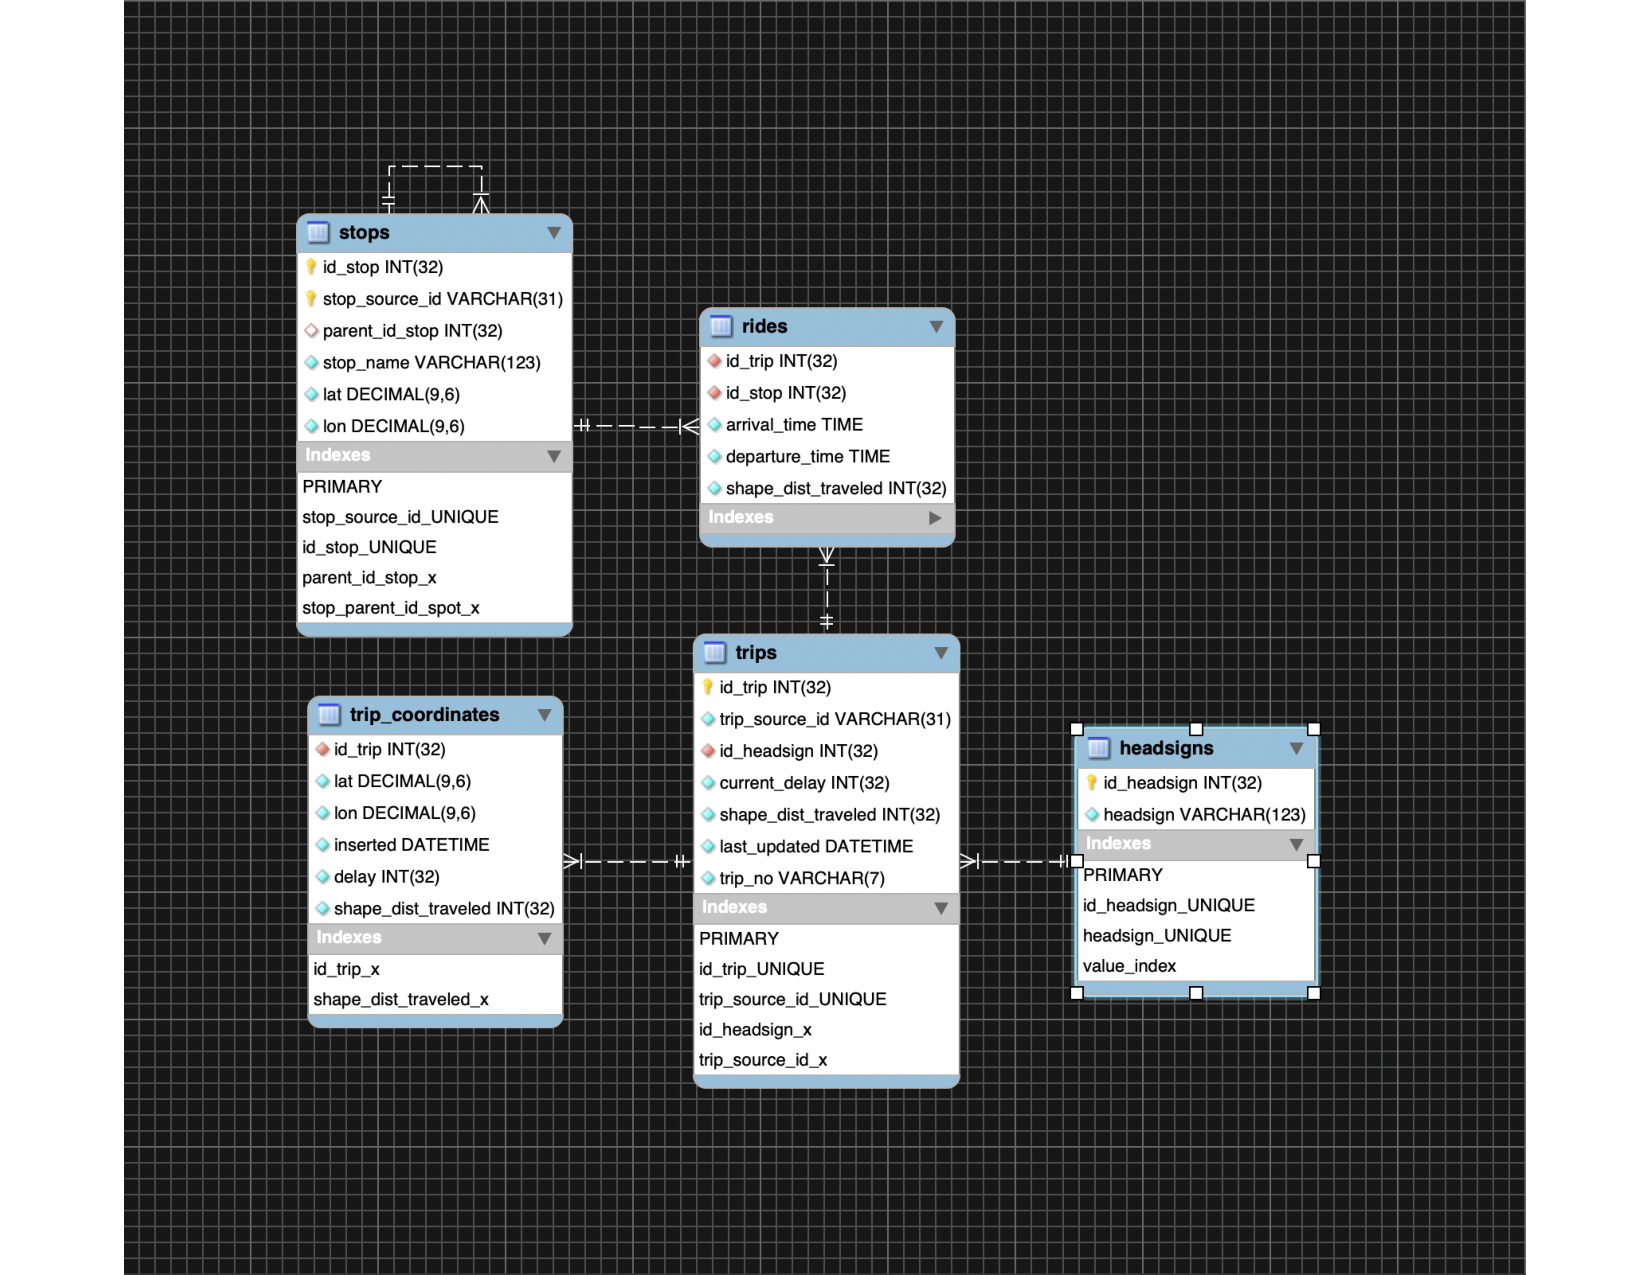
\includegraphics[width=\linewidth]{../img/eer_database}
% Příponu není potřeba explicitně uvádět, pdflatex automaticky hledá pdf.
% Rozměry také není nutné uvádět.
\caption{EER diagram databáze.}
\label{obr:EER}

\end{figure}

\begin{itemize}
	\item \verb-trips- všechny objevené jízdy

		\begin{itemize}
			\item \verb-id_trip- unikátní identifikátor používaný v databázi

			\item \verb-trip_source_id- identifikátor tripu převzatý ze zdroje dat

			\item \verb-id_headsign- identifikátor nápisu pro daný trip

			\item \verb-current_delay- aktuální zpoždění tripu

			\item \verb-shape_dist_traveled- aktuální vzdálenost ujetá od výchozí stanice

			\item \verb-last_updated- čas poslední aktualizace, převzatý ze zdroje dat

			\item \verb-trip_no- číslo dané linky
		\end{itemize}

	\item \verb-headsigns- nápisy nad vozidlem, cílová stanice

		\begin{itemize}
			\item \verb-id_headsign- unikátní identifikátor nápisu

			\item \verb-headsign- text nápisu
		\end{itemize}

	\item \verb-trip_coordinates- všechna historická real-time data

		\begin{itemize}
			\item \verb-id_trip- identifikátor tripu, ke kterému se záznam váže

			\item \verb-lat- zeměpisná šířka polohy vozidla

			\item \verb-lon- zeměpisná délka polohy vozidla

			\item \verb-inserted- čas vložení záznamu

			\item \verb-delay- zpoždění zachycené v poslední projeté stanici před pořízením záznamu

			\item \verb-shape_dist_traveled- vzdálenost ujetá od výchozí stanice tripu

		\end{itemize}

	\item \verb-stops- všechny zastávky

		\begin{itemize}
			\item \verb-id_stop- unikátní identifikátor zastávky

			\item \verb-trip_source_id- identifikátor zastávky převzatý ze zdroje dat

			\item \verb-parent_id_stop- identifikátor rodičovské zastávky, pokud existuje

			\item \verb-stop_name- název zastávky

			\item \verb-lat- zeměpisná šířka polohy zastávky

			\item \verb-lon- zeměpisná délka polohy zastávky

		\end{itemize}

	\item \verb-rides- trasa každého tripu, seznam zastávek s časy odjezdů a příjezd tvořící jízdní řád, relační tabulka mezi spoji a zastávkami, pořadí zastávek v jakém jsou spojem obslouženy je určeno časem příjezdu resp. odjezdu tak i atributem \verb-shape_dist_traveled- \label{table:rides}'

	\begin{itemize}
		\item \verb-id_trip- identifikátor tripu

		\item \verb-id_stop- identifikátor zastávky

		\item \verb-arrival_time- čas příjezdu tripu do zastávky

		\item \verb-departure_time- čas odjezduu tripu ze zastávky

		\item \verb-shape_dist_traveled- vzdálenost zastávky od výchozí zastávky tripu

	\end{itemize}

\end{itemize}

Atributy se jménem *source\_id jsou pravděpodobně unikátní identifikátor entity ve zdroji dat, nicméně z dokumentace zdroje to nevyplývá. Také je tento indenfikátor ukládán jako textový řetězec, ačkoli je tvořen pouze číslicemi a podtržítky, není nikde zaručeno, že jej lze jednoduše převést na číselný ko'd. Takže pro lepší výkon databáze je použito automaticky generované id typu \gls{int}.

\bigbreak

Každá tabulka má několik indexů, které zlepšují výkon databáze při vkládání a hledání dat. Obvzláště pokud je atribut označen jako unikátní, kde se při každém vložení ověřuje unikátnost.

\bigbreak

Databáza je nastavená tak, aby umožňovala získat všechny potřebné informace o vozidlech, ale hlavně přístup k historickým real-time datům a to separovaně pro dvojci refenčních bodů. K tomu se zejména využívá atribut \verb-shape_dist_traveled-, který označuje vzdálenost na trase od výchozí zastávky a je součástí vstupních dat jízdních řádů i aktuálních poloh vozidel.

\subsection{Plnění databáze}

Tato databáze bude plněna skriptem, jehož bude naprogramován taky, aby vždy stáhl aktuální obraz dopravní situace a tato data uložil do dotabáze. Toto stahování z datové platformy probíhá podle násldujícího algoritmu.

\bigbreak

Algoritmus:
\begin{code}[frame=none]
načti všechny dostupné zastávky
dokud skrip běží
  načti aktuální polohy vozidel
  pro každé nalezené vozidlo
  pokud jízda vozidla je známá
    aktualizuj data o jízdě
  jinak
    stáhni informace o jízdě
    zpracuj a vlož jízdu do databáze
\end{code}

\bigbreak

Protože všechny infomace ukládané do databáze jsou důležité pro hlavní cíl této práce, tak pokud se vyskytne jízda, který neobsahuje některou z požadovaných infomarcí je pak automaticky zahozena. To je řešeno pomocí databázových transakcí tak, aby stav databáze byl vždy konzistentní. Transakce v obecném smyslu fungují tak, že můžeme měnit data v databázi (i více zázanamů) a tyto změny se zapíší do samotné databáze až po potvrzení, že všechny změny byly provedeny správně, pokud během provádění změn nastane chyba, můžeme v jakékoli fázi provádění změn všechny dosud proveedné změny zahodit a vrátit se do původního stavu databáze před započetím transakce.  Tedy pokud nejsou poskytnuta data ve formátu, který skript akceptuje, nebo nějaké povinné atributy chybí. Vložení celé jízdy nebude provedeno.

\bigbreak

Nejčastěji chybějící atribut je zpoždění v poslední zastávce, toto je nutné vědět pro počítání zpoždění mezi refenrečními body (zastávkami). Absence této informace může být způsobena tím, že vozidlo vůbec nevysílá data potřebnák k jejím dopočtení, pak nemá smysl jej do databáze zahrnovat. Nebo vozidlo už vysílá, ale ještě nezahájilo jízdu, tedy nemá žádnou poslední projetou zastávku, v takovém případe budou data ignorována až do doby příchodu první relevantní informace.

\bigbreak

Mimo popsanou databázi se do určeného adresáře ukládají trasy jednotlivých jízd, která jsou ve fromátu \gls{geojson} jako lomená čára definována souřadnicemi. Navíc data o trasách jsou používána pouze pro vizualizaci a jsou přijímány vizualizačním nástrojem ve formátu \gls{geojson}, tedy tyto data není nutné vůbec transformovat a není nutné je držet v hlavní databázi.

\bigbreak

 Stejně tak i aktuální polohy vozidel jsou mimo databázi zapisovány do souboru, který je určen a formátován pro čtení webovou aplikací. Aktualizace tohoto souboru je provedena přednostně, ihned po načtení real-timových dat. Tím se zabrání nechtěnému čekaní na aktualizaci celé databáze, která může trvat jednotky sekund.









\section{Algoritmus odhadu zpoždění}

Z toho jak je problém formulován vyplývá, že se má odhadovat zpoždění mezi dvěma refenčními body a jediné takové jsou zastávky na trase danného spoje. Proto cíl algortimu může být formulován, jako vytvořit popis průběhu trasy mezi každou dvojcí zastávek, které alespoň jeden spoj obsluhuje a jsou bezprostředně sousedící ve sledu zastávek ve směru jízdy tohoto spoje. Nechtˇ se všechny dvojce zastávek a spoje je obsluhůjící splňující předcházející předpoklad označují jako $AB$ a $S$. Jedda dvojice zastávek pak bude $(a, b)$ a spoje je obsluhující se značí jak $S_{ab}$.

\bigbreak

Z definice problému chceme modelovat jízdu vždy mezi danou dvojcí zastávek. Ke každé dvojci zastávek $(a, b)$ bude náležet jeden model, popisující průběh jízdy mezi nimi. Tyto modely budou vycházet z historických dat průjezdů mezi těmito zastávkami.

\bigbreak

Příklad takové dvojce zastávek $a$ a $b$ je uveden na příkladu v kapitole \ref{subsection:priklad_nelinearni_trasa}.

\subsection{Základní předpoklady} \label{section:zakladni_predpoklady}

Hned na začátek je potřeba ustanovit základní předpoklady, ze kterých bude vycházet sestrojený algoritmus vytvářející modely profilů jízd.

\bigbreak

Zastávky je potřeba rozlišovat na jednotlivá nástupiště. Toto výrazně nezvýší počet dvojic zastávek $AB$. Protože naprostá většina zastávek má pouze dvě nástupiště\footnote{Rozepsáno v kapitole \ref{subsubsection:zastavky}}. Pro každý směr jedno. Pokud má více nástupištˇ, pak tak bývá v případech, kdy ze zastávky odjíždí spoje do více směrů a tudíž pro každné nástupiště je jiná následující zastávka -- počet dvojic $(a, b)$ se nezvýší. Z toho plyne zjednodušení, kterého se dopouštíme v průběhu celé práce, především pak pro tento algoritmus ohadu zpožění a to, že termíny zastávka a nástupiště splývají.

\bigbreak

Všechny spoje $S_{ab}$ bez ohladu na linku nebo dopravce jedou ze zastávky $a$ do zastávky $b$ po stejné trase a tedy vzdálenost je konstatní. -- Předpokládá se, že žáný dopravce nevyužívá jinou komunikaci a pro všechny platí pravidla silničního provozu stejně.

\bigbreak

Čas jízdy ze zastávky $a$ do $b$ závisí pouze na denní době a dne v týdnu. Navíc platí žádný z dopravců nedisponuje právem přednosti v jízdě před jiným dopravcem nebo výrazně výkonějším vozidlem.  Dojezdové časy mohou být ovlivněny jen charakterem řidiče, avšak toto není zjistitelné z poskytnutých dat a zároveň se předpokládá, že charatery řidičů jsou rovnoměrně rozloženy mezi všechny dopravce a linky. Podle jízdních řádů některé linky jedou ve stejnou denní dobu rychleji než jiné, avšak skutečné doba jízdy je stejná. To že některý spoj zastávku projíždí a tím je rychlejší než jiný spoj není porušení tohoto předpokladu protože se jedná o dvě různé dvojce zastávek.

\bigbreak

Během jízdy mohou nastat mimořádnosti, které porušují výše uvedené předpoklady, nicméně detekce mimořádností a jejich řešení je nad rámec této práce a jejich počet je zanedbatelný, proto na statistické modely nebudou mít vliv.

\subsection{Analýza dat a návrh modelování} \label{subsubsection:analyza_dat}

Na úvod uvedˇme, že ve všech grafech a následně pro počítání modelů byly všechny zobrazené vzorky poloh vozidel v grafech zarovnány tak, aby jejich jízda ze zastávky $a$ vždy začínala se spožděním 0 sekund. To podle nahlášeného zpoždění v zastávce $a$.

\bigbreak

Z dat je však patrné, že né vždy se zarovnání do nuly podařilo. Takové případy jsou pak způsobeny chybamy v datech vysílaných z vozidel nebo špatně určeným zpožděním v poslední projeté stanici na straně dodavatele dat. Takové chyby však vznikají spíše vyjímečně a proto ovlivnˇují statistické výpočty jen málo. Pro eliminaci těchto chyb je pak v implementován modul, který se pokouší očividně chybné vzroky najít a smazat. To primárně z důvodů vizualize vzorků v grafech, kde jeden vzorek zcela mimo škálu jiných vzorků rozhodí celý graf a graf se tak stává nepřehledným.

\subsubsection{Lineární model}


Odhad zpoždění vozidla na trase se v současné době provádí pomocí lineárního modelu. Tedy s předpokladem, že vozidlo jede konstatní rychlostí po celou dobu jízdy mezi dvojcí zastávek $a$ a $b$.

\bigbreak

Ačkoli je snaha tento model nahradit lepším, v některých situacích může jeho použití i na dále dávat smysl. Zejména pak v případech kdy není k dispozici dostatek dat a nebo je vzdálenost dvou zastávek natolik malá, že nemá smyl ani jakýkoliv odhad zpoždění dělat. (TODO do problemu: Lepší by bylo volit trasy s nejmenší dobou jízdy, ale čas jízdy je promněnlivý a težko se získá skutečná doba jízdy z dat. Navíc v praxi jsou vzdálenost a doba jízdy dostatečně závislé)

\subsubsection{Polynomiální profil jízdy}

Po analýze dat poloh vozidel a možných vlivů ovlivnˇující profil jízdy je patrné, že v průběhu jednoho dne dochází na trase nejvýše k několika výkyvům rychlosti jízdy. Viditelné jako "vlny" v průběhu dne na grafu \ref{fig:dojezd_ve_fazich_dne}), v 8:30 hod\footnote{časy jsou uvedeny v UTC}. jízda trvala téměř 10 minut, naopak ve večerních hodinách jízda trvá kolem 7 minut.

\bigbreak

K tomuto dochází například v případech kdy spoj zastavuje ve městě a v následujících několika málo kilometrech jede pomaleji, poté zrychlý a dále opět vjede do města. Takový model se hodí spíše na delší trasy s plynulou jízdou.

\begin{figure}
	\centering
  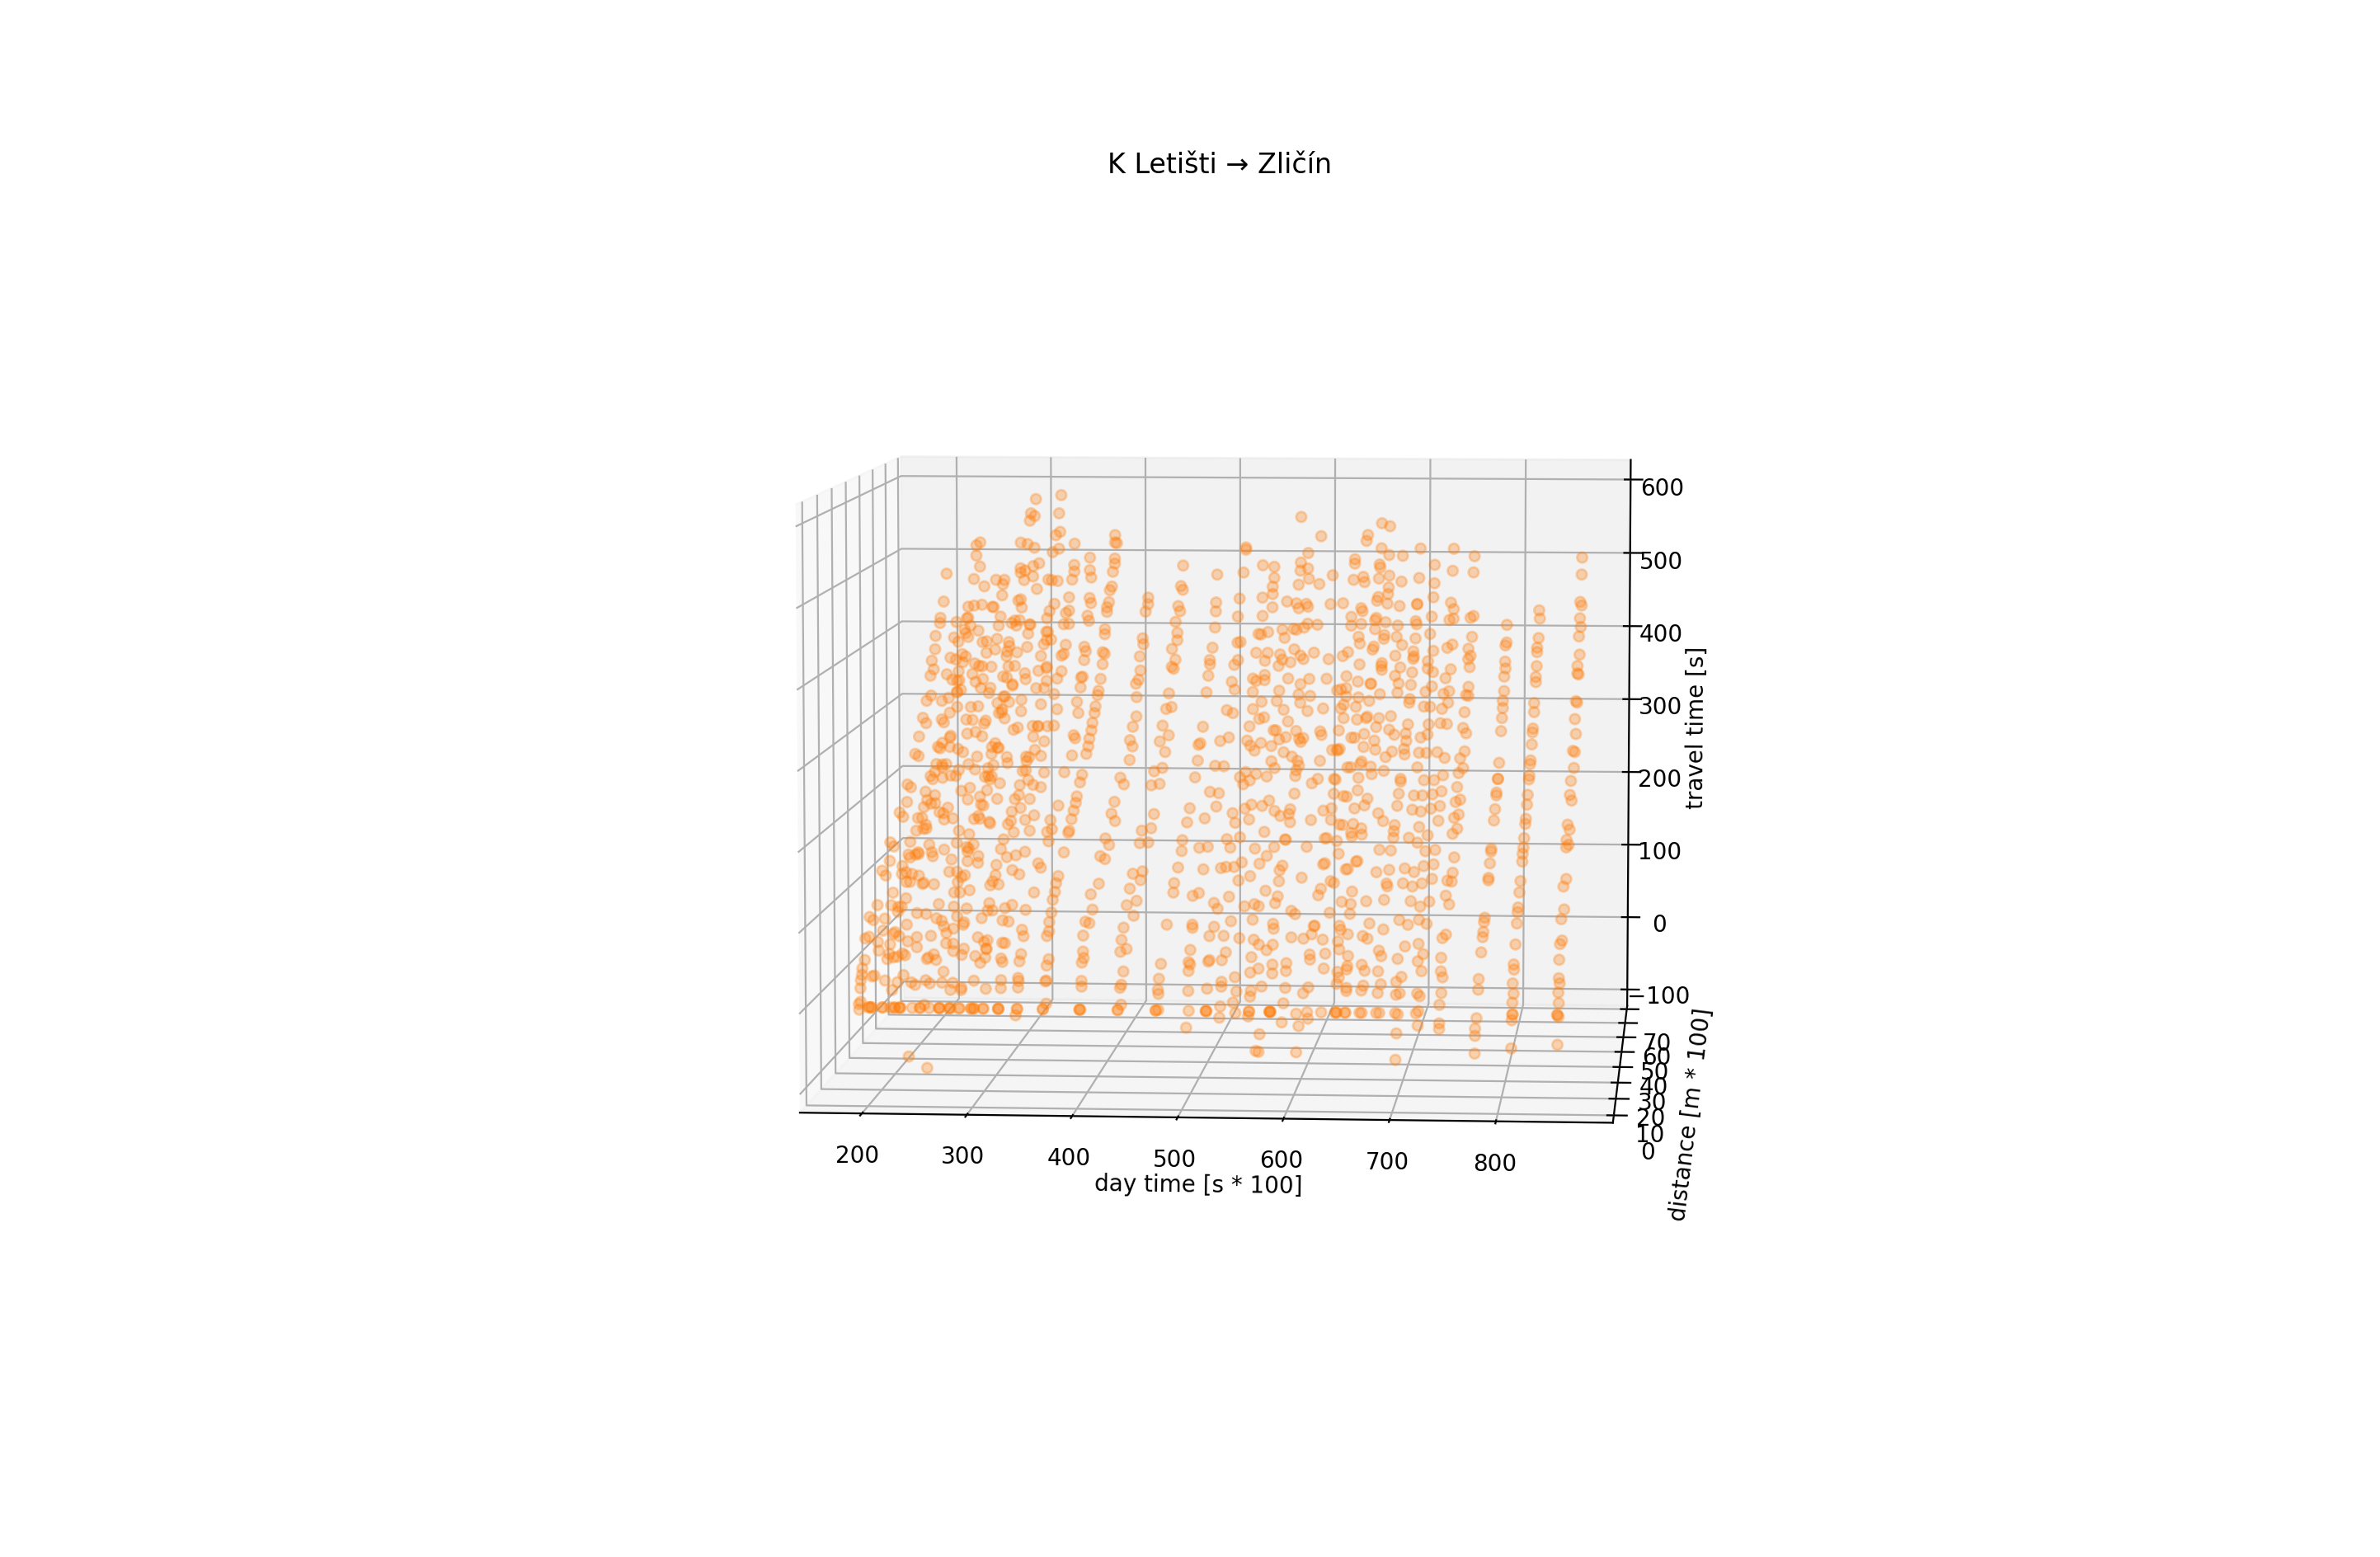
\includegraphics[width=\linewidth]{../img/dojezd_ve_fazich_dne.png}
  \caption{Variabilita délky jízdy v průběhu dne}
  \label{fig:dojezd_ve_fazich_dne}
\end{figure}

Stejně tak po analýze profilu jízdy vzávislosti na ujeté vzdálenosti je na grafu \ref{fig:dojezd_podle_vzdalenosti} vidět, že čas jízdy narůstá taky v jistých "vlnách".

\begin{figure}
	\centering
  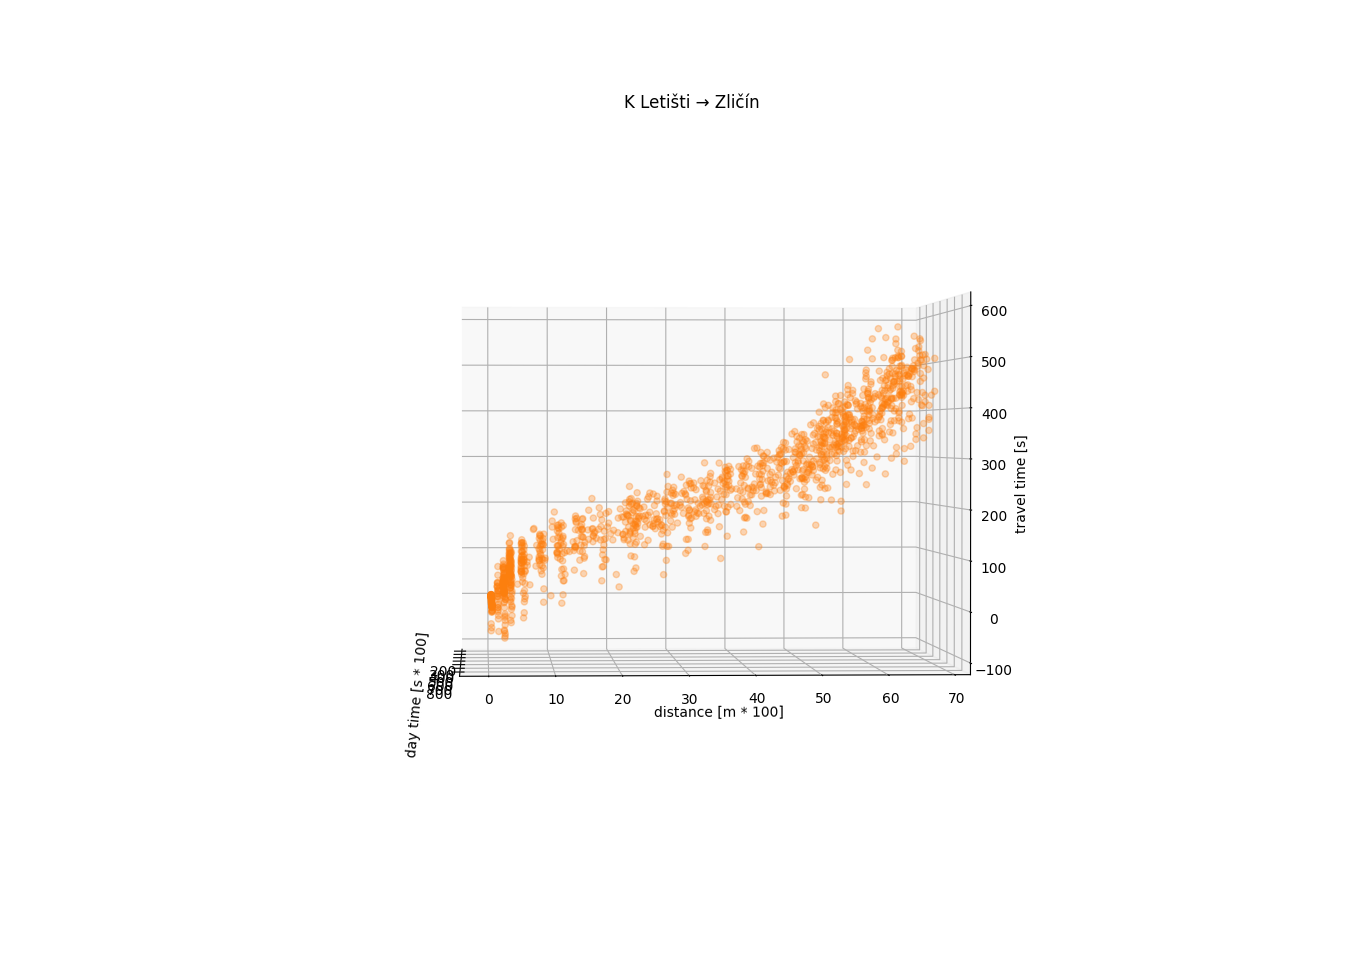
\includegraphics[width=\linewidth]{../img/dojezd_podle_vzdalenosti.png}
  \caption{Variabilita času jízdy v závislosti na ujeté vzdálenosti}
  \label{fig:dojezd_podle_vzdalenosti}
\end{figure}

Podle charakteru těchto dat nejlépe budou odpovídat modely získané pomocí lineární regrese, resp. polynomiální regrese.

\bigbreak

Jako odhad zpoždění se pak vrací rozdíl skutečného počtu sekund na trase a predikce modelu. To celé se pak ještě přičítá k rozdílu predikce v modelu v čase a vzdálenosti příjezdu podle jízdního řádu a pravidelného příjezdu.

\bigbreak

Polynomiální model se tedy hodí pro situace kdy je průběh trasy nějak ovlivněn vždy ve stejném úseku a má vliv na každý projíždějící spoj. Nebo se v průběhu dne pozvolna mění v závislosti na dopravním vytížení projížděných úseků.

Polynomiální model je pro představu vykreslen v grafu v úvodním příkladu v kapitole \ref{subsection:priklad_nelinearni_trasa}.

\subsubsection{Nepravidelné profily jízdy}

Výše popsaný příklad však ilustruje téměř ideální případ, kde je pravidelnost jízdy velmi dobře viditelná. Rozeberme si proto nyní i jiné druhy profilů jízd.

\bigbreak

Na grafu \ref{fig:cerny_most_chvaly} je patrné, že vzorky poloh vozidel profilu jízdy stále vytváří vlny. Ovšem už nejsou tak jednoznačně vidět jak v předchozím příkladě a především se v celém grafu objevuje pár vzorků, které zcela vybočují mimo největší zhluky vzorků. V těchto případech se, ale zřejmě jedná o případy vozidel, které potkala nějaká anomáli při výjezdu ze stanice a proto nabraly zpoždění hned na začátku.

\begin{figure}
	\centering
  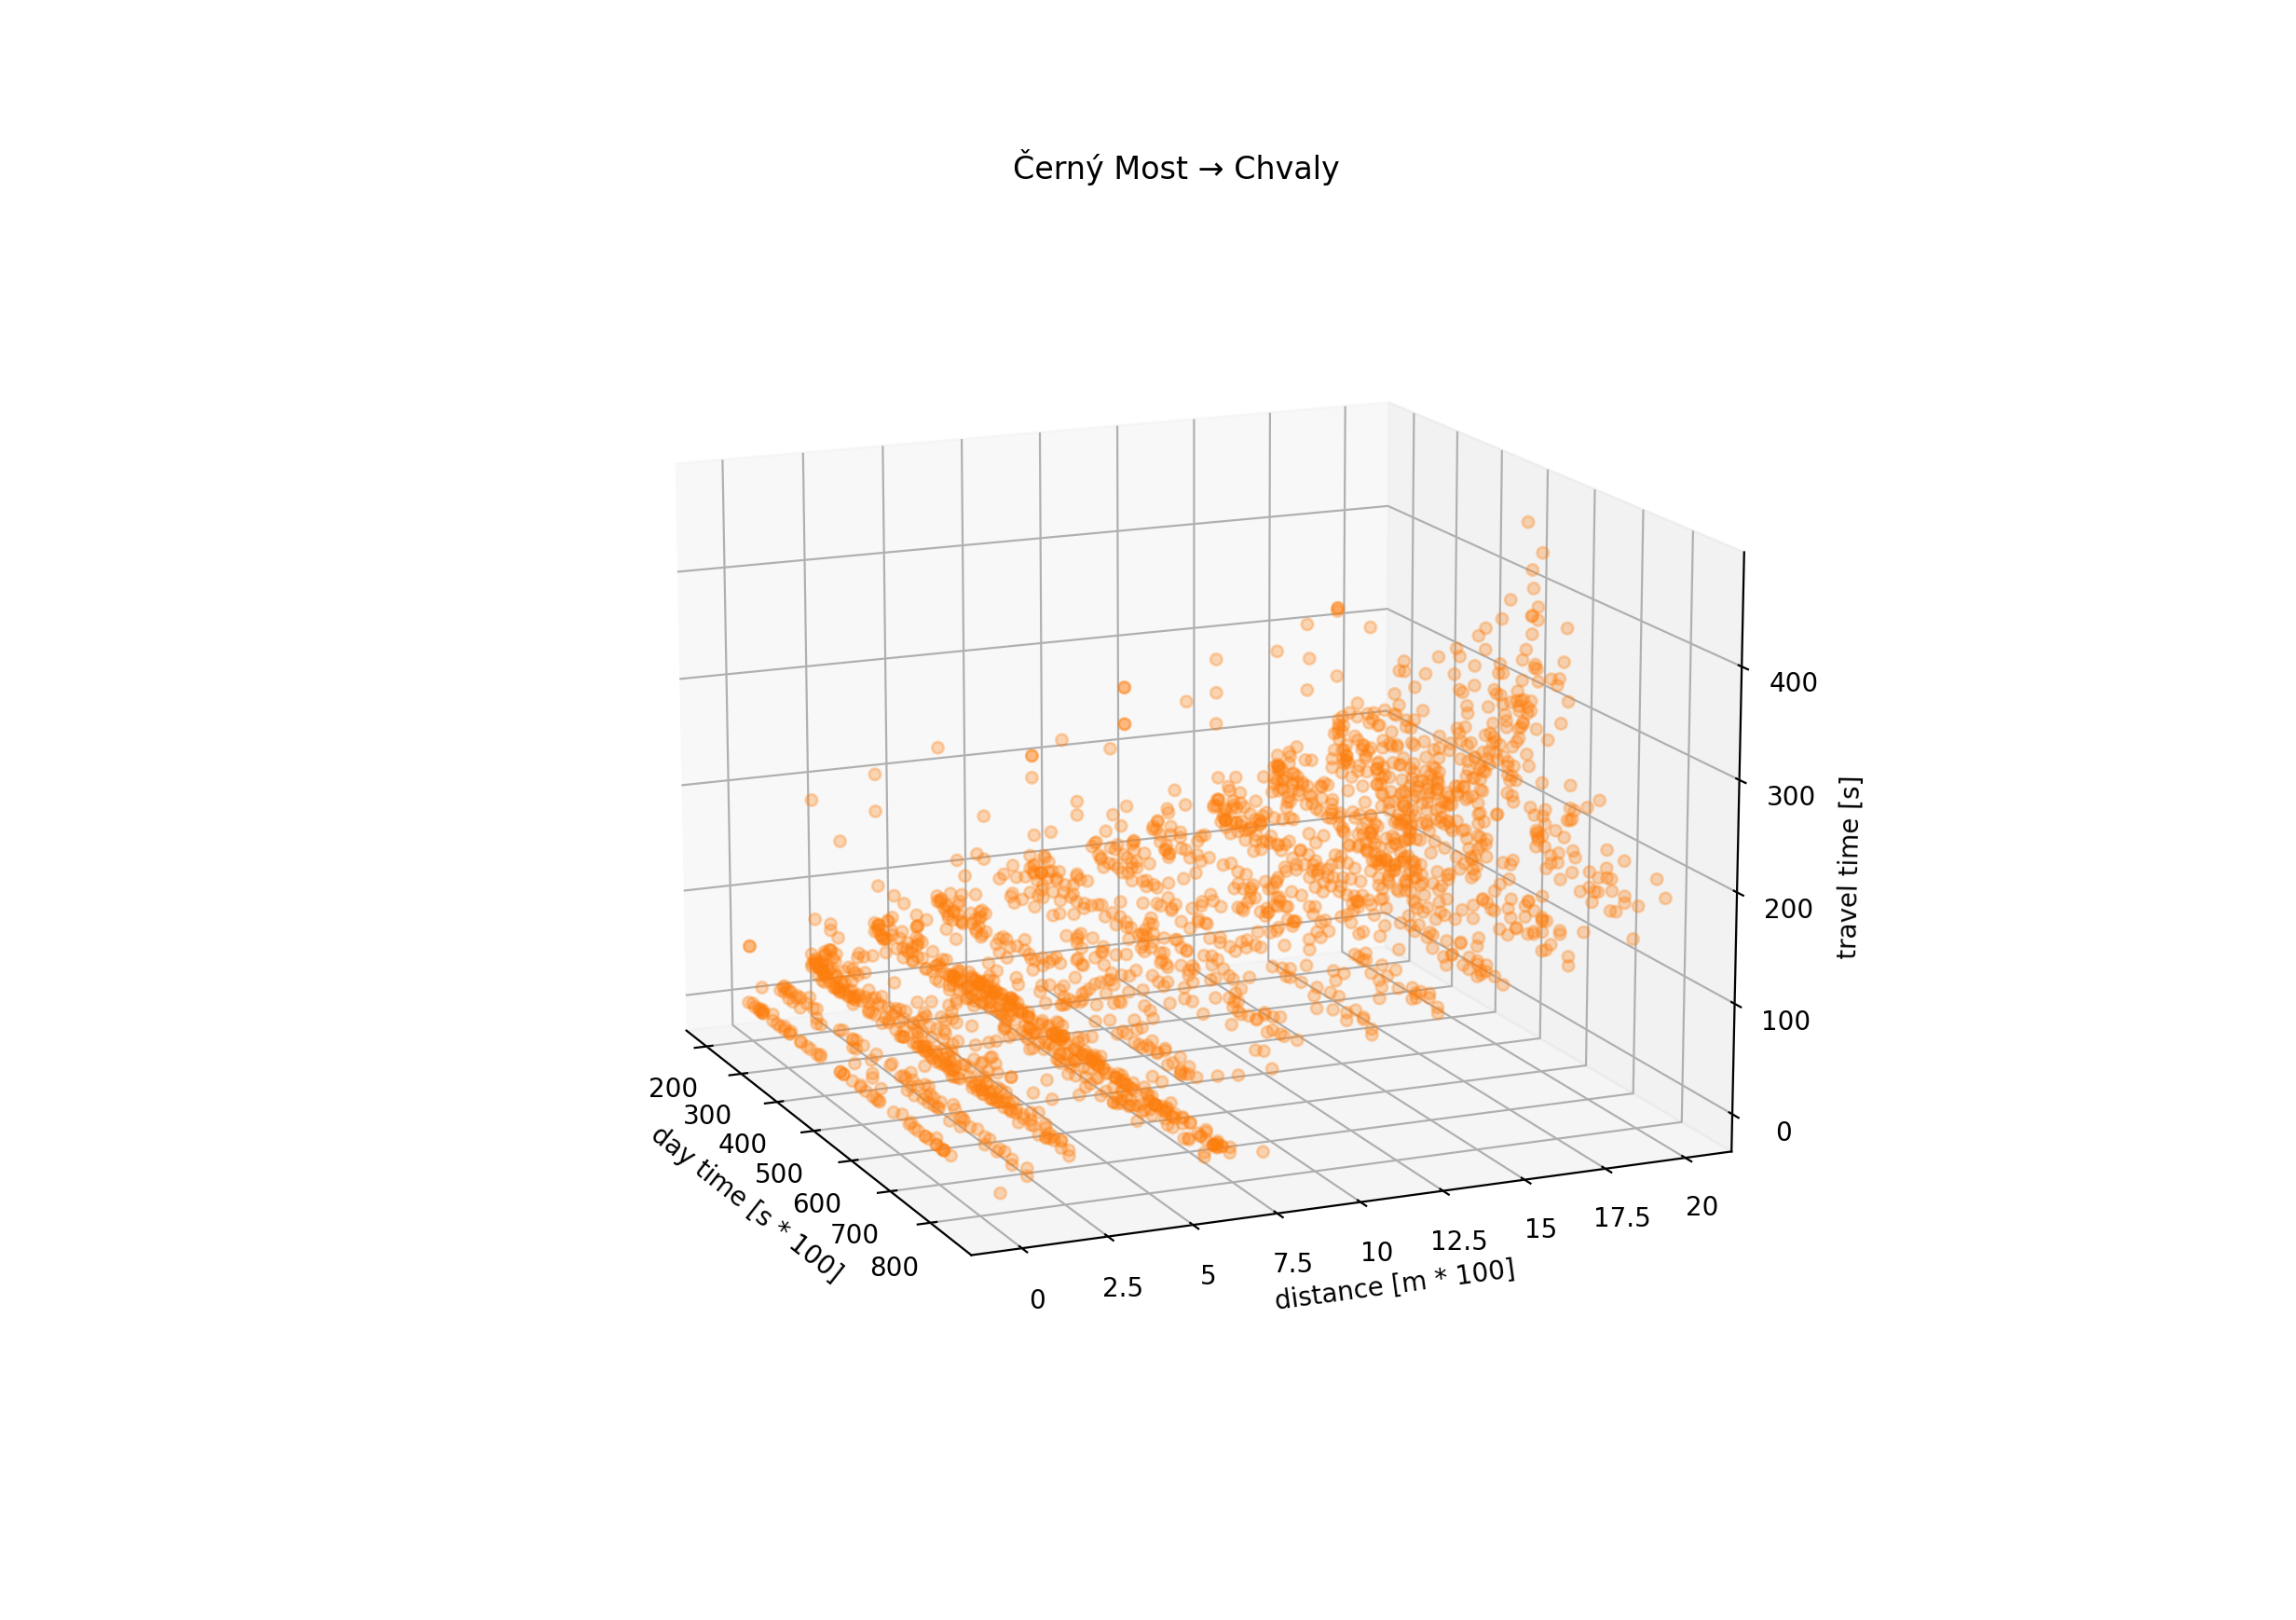
\includegraphics[width=\linewidth]{../img/cerny_most_chvaly.png}
  \caption{Úsek s nepravidelnostmi}
  \label{fig:cerny_most_chvaly}
\end{figure}

Pro velmi krátké trasy se zobrazené vzorky dat mohou jevit jako zcela nepravidelné. Příklad uveden na grafu \ref{}. To je způsobeno tím, že doba jízdy trasy je natolik krátká, že jeden spoj trasu projede za minutu, ale druhý sopj, který se zdrží o zanedbatelný čas (z pohledu problému řešeného v této práci) přijede do následující stanice až za dvoujnásobou dobu. Dále je vysoký rozptyl vzorků způsoben nepřesnostma při měření polohy vozidel a dalších možných problémů. Jelikož se ale jedná o velmi krátké trasy nemá smysl jejich specifka vůbec řešit, protože spočítaná data by zastarala ještě před zveřejněním.

\begin{figure}
	\centering
  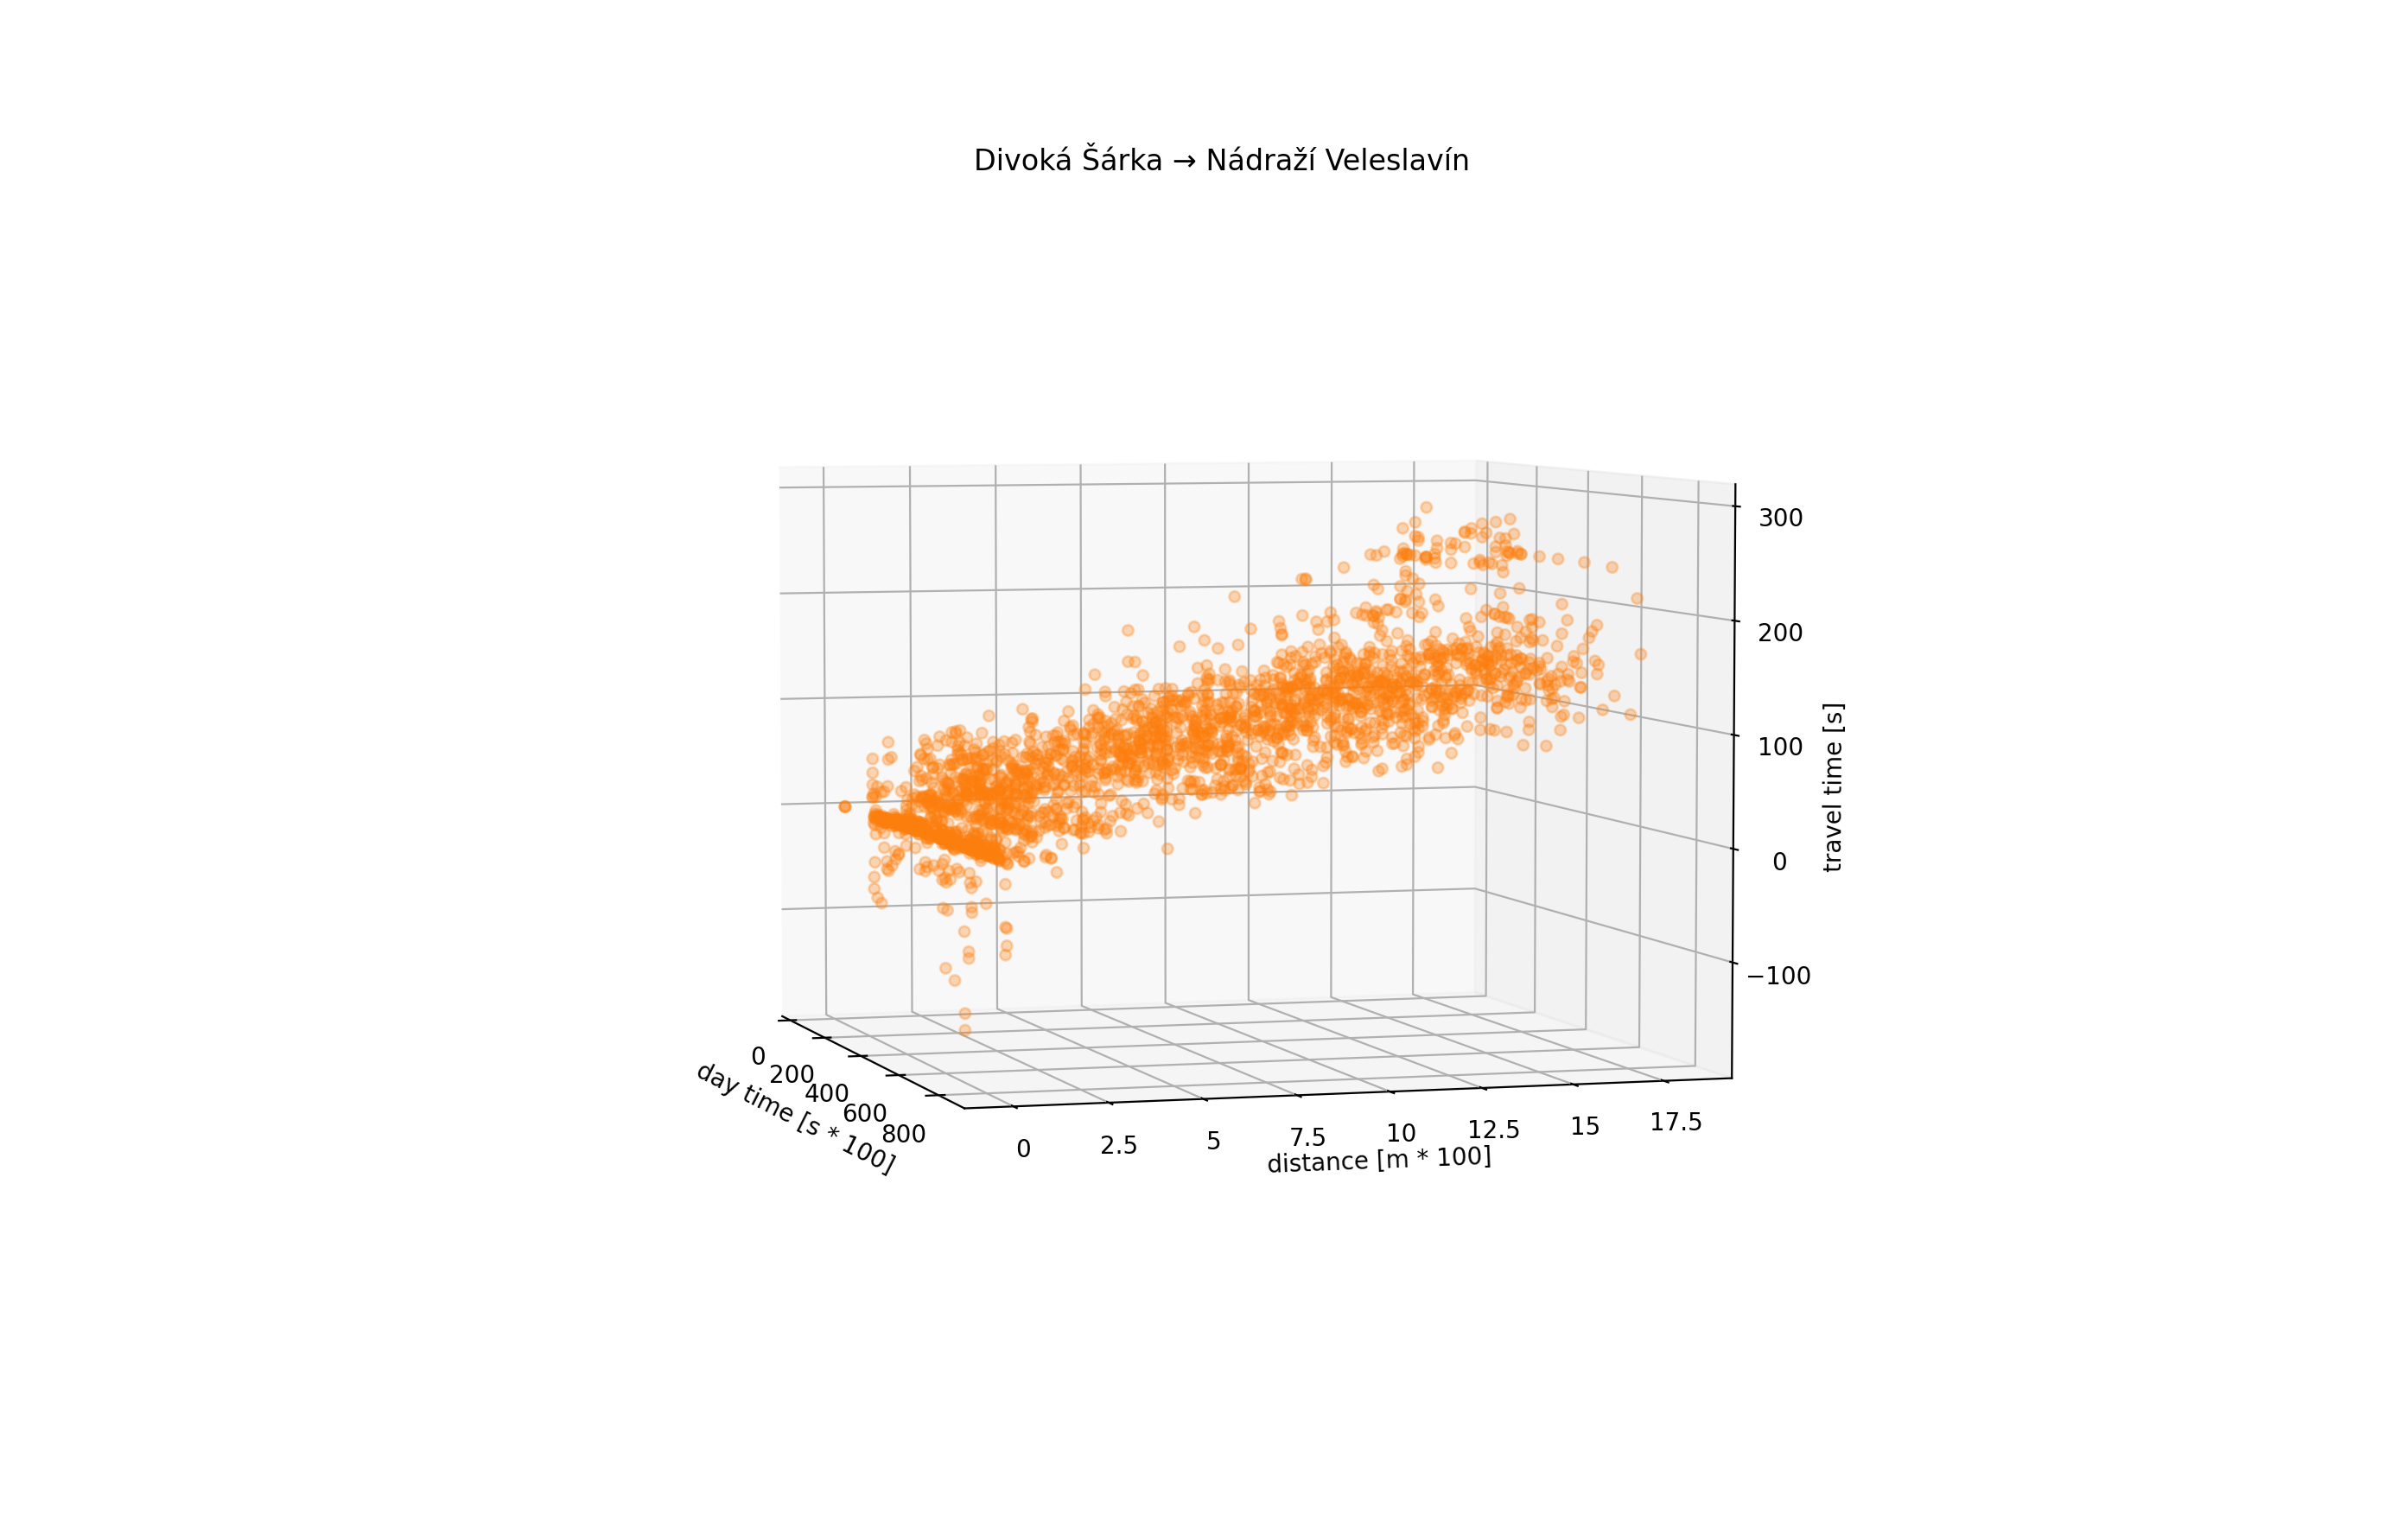
\includegraphics[width=\linewidth]{../img/divoka_sarka_veleslavin.png}
  \caption{Úsek s nepravidelnostmi 2}
  \label{fig:divoka_sarka_veleslavin}
\end{figure}

\subsubsection{Model konkávním obalem}

Na dalším grafu \ref{fig:nepredvidatelne_zdrzeni} je zobrazen příklad, kdy na trase exituje bod, který určité procento projíždějících spojů zdrží o netriviální dobu. Něco takového nastane, pokud spoje projíždí světelnou křižovatkou nebo místem kde se náhodně tvoří kolona vozidel. Zde dochází ke skové změně průběhu bodové funkce. Spojité modely, jakým je polynomílní model, by s okolím tohoto kritického místa měly problém. Pro případy, kdy je na trase jen jeden takový bod by použití polymoniálních modelů vyhovovovalo, bytˇ by v bodě skoku odhad nebyl úplně přesný, ale předpokládejme, že nalezená polynomiání funkce by tento skok zohlednila. Ale teroreticky je potřeba algoritmus, který umí pracovat s více kritickými body na trase.

\begin{figure}
	\centering
  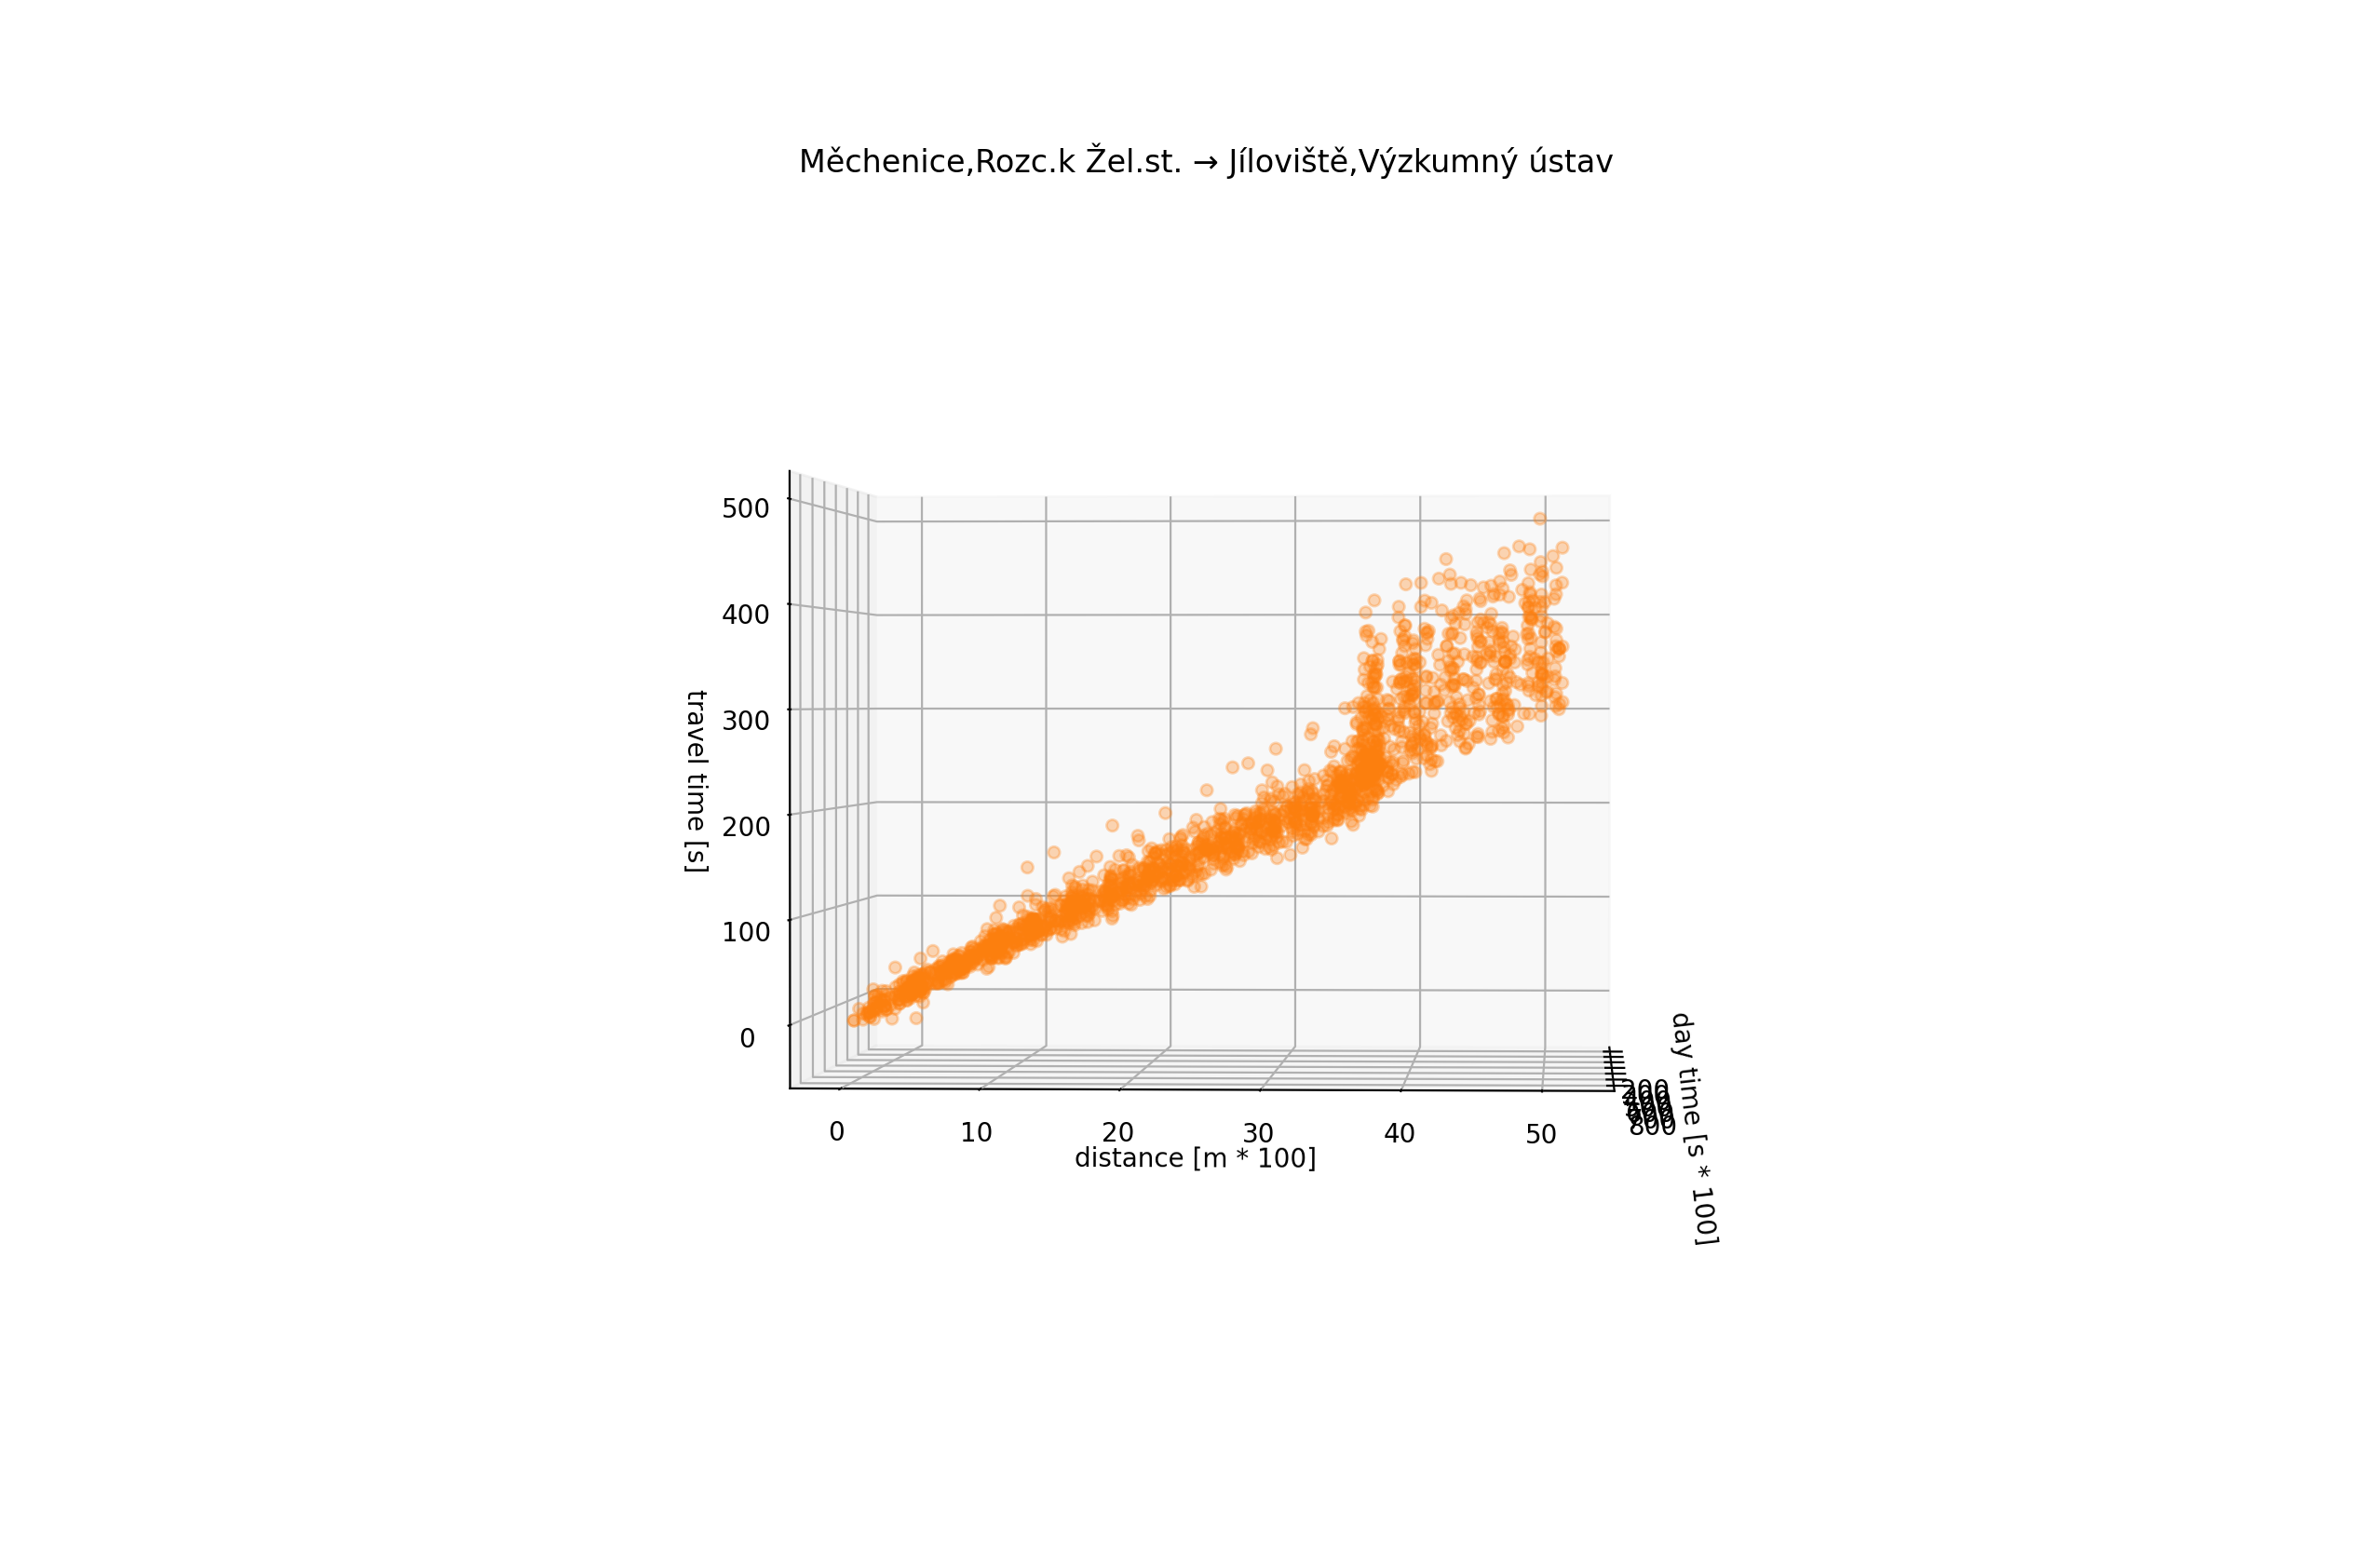
\includegraphics[width=\linewidth]{../img/nepredvidatelne_zdrzeni.png}
  \caption{Úsek s nepravidelnostmi}
  \label{fig:nepredvidatelne_zdrzeni}
\end{figure}

Nevyhovující průběh trasy se dvěma kritickými body $x$ a $y$ na trase odpovídá následně popsané modelové situaci jízdy vozidel mezi dvěma zastávkami. Uvažume, že se většina projíždějících spojů zdrží pouze v prvním kritickém bodě $x$ o $c$ sekund, nebo pouze v druhém kritickém bodě $y$ o $c$ sekund, nebo se lehce zdrží v obou kritických bodech o $c_y + c_x = c$ sekund\footnote{$c_x$ značí nabrané zpoždění v bodě $x$, pro $y$ analogicky}. S takovým zdržením je počítáno v jízdním řádu a tedy vozidla, která projedou první kritický bod bez zdrření jedou na čas stejně tak, jako vozidla v něm zdržená. O snížení nebo zvýšení případného zpoždění spoje je možno rozhodnout až po projetí druhého bodu. Zatímco polynomiální model by svými odhady jen uváděl uživatele v omyl.

\bigbreak

Jinými slovy na grafu času jízdý a vzdálenosti od vyjetí ze zastávky vzniká jakýsi podprostor v němž se zpoždění nemění. Pro ohraničení tohoto podprosoru je potřeba sestrojit konkávní obal všech vzorků všech spojů, které přijely do následující zastávky včas.

\bigbreak

Nejprve k samotnému konkávnímu obalu je potřeba říct, že na množině bodů není definován jednoznačně, jak je vidět na obrázku \ref{fig:konkavni_obal_nejednoznacny}\footnote{Zdroj: Alpha-Concave Hull, a Generalization of Convex Hull, Saeed Asaeedi, Farzad Didehvar, and Ali Mohades, Department of Mathematics and Computer Science, Amirkabir University of Technology, https://arxiv.org/pdf/1309.7829.pdf}. Pro úšely této práce je zapotřebí spočítat obal ve třídimenzionálním prostoru, což je velmi komplikovaný úkol, a není ani snadné nalézt knihovny, které by konkávní obal ve 3D spočítaly. a proto je potřeba přijít s zjednodušením úlohy. Tedy počítat obal pouze pro dvoudimenzionální prostor. Toho se nedá dosáhnou jinak než diskretizací úlohy a počítání obalu pro každou hodinu zvláštˇ, tedy ze všech bodů, které byly zaznamenány v průběhu jedné hodiny.

\begin{figure}
	\centering
  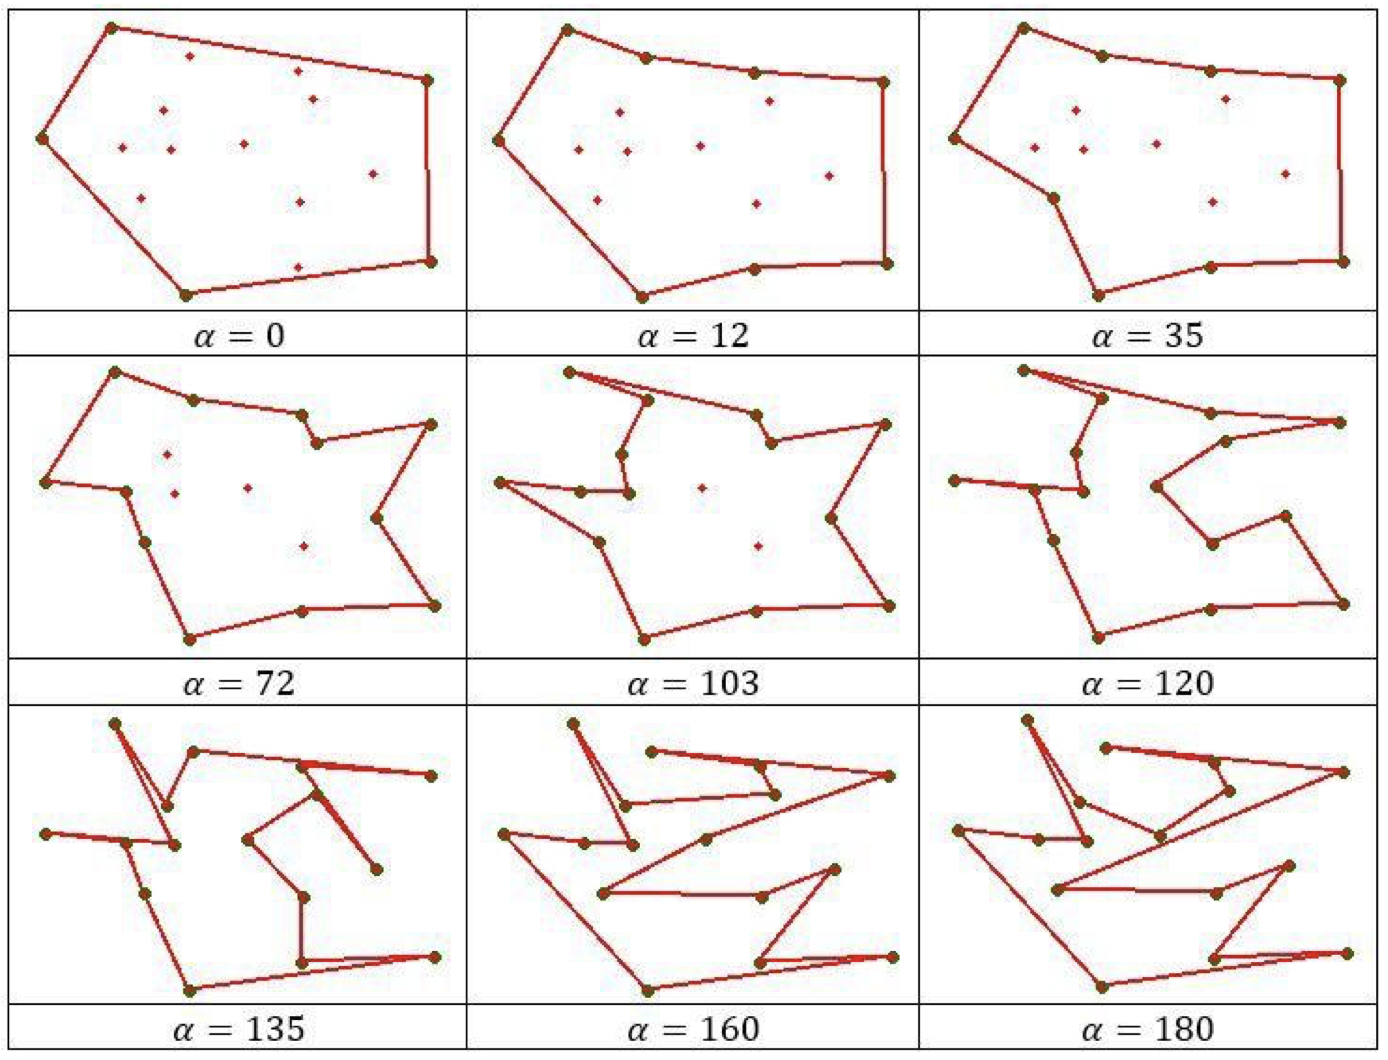
\includegraphics[width=0.8\linewidth]{../img/konkavni_obal_nejednoznacny.png}
  \caption{Nejednoznačnost konkávního obalu}
  \label{fig:konkavni_obal_nejednoznacny}
\end{figure}

 Tím může dojít k vetší granularitě obalu, než by bylo vhodné, nicméně předpokládá se, že hodina je dostatečně dlouhý časový interval na to, aby zde byly zachyceny všechny druhy průběhu jízdy a zároveň je to dostatečně krátký interval na nezkreslování denních výkyvů v čase jízdy.

 \bigbreak

Dále se jako netriviální ukazuje detekce spojů, které přijely včas a tedy všechny jejich body mají být předány k výpočtu obalu. Nabízí se použít data o všech spojí, které přijely do cílové zastávky s co nejmenším zpožděním, ale je nutné mít na paměti, že příjezdy podle jízdního řádu nemusí vůbec odpovídat realitě. Proto se zdá být nejlepší použít data od spojů, které přijely ve stejnou dobu jako je průměr všech příjezdů do cílové zastávky. Toho se docílí tak, že se poslední vzorky podle vzdálenosti všech spojů použijí pro odhad času příjezdu. Dále se pro každou hodinu použije se určité procento nejbližších spojů k tomuto odhadu.

\bigbreak

Z předchozího popisu řešení vyplývá ovšem, že pro výpočet obalu jsou použity spoje, které ani zdaleka nemusely přijet včas jak je požadováno, ale předpokládá se, že se nepříliš vzdalují od průměrného času příjezdu. To že střední zpoždění pro celý obal není nulové se vyřeší spočtením odchylky průměrného příjezdu od příjezdu podle jízdního řádu a následně přičtení této konstanty k odhadnutnému zpoždění. Každopádně to, že rozptyl příjezdů spojů zahrnutých ve výpočtu obalu může být netriviální, vyžaduje nahlížet na tento obal jako na lineární prostor pohybu zpoždění. Tedy že odhad zpoždění pro bod nacházející se v obalu je lineárně závislý na vzdálenosti od hranice obalu, avšak protože je známo časové rozpětí příjezdu spojů použitých pro výpočet obalu, je možné tuto vzdálenost snadno přenést na skutečné pozdění.

\bigbreak

Naštěstí pro nás se v průběhu analýzy dat o polohách spojů nepodařilo najít jediný případ dvojce zastávek, mezi kterýma by došlo k popsané situaci -- výskytu dvou kritických bodů. Nebo tyto body jsou natolik nevýrazné, že by popsané řešení pomocí konkávního obalu nepřineslo žádné zlepšení odhadu zpoždění, ba naopak vzhledem k implementační náročnosti a množstvím chyb vznikajícím při tak algoritmicky náročných úkolech by přesnost odhadu zpoždění zhoršilo. Možných vysvětlení proč tato situace nenastává se nabízí více. Zejména vlivem složitosti dopravní sítě a závsilostí v ní je možné, že pokud se vozidlo zdrží v jedné koloně vozidel a na jeho trase se ještě jeden kritický bod, pak je velmi pravděpodobné že se zdrží i v něm, protože hustota dopravy je ve stejném čase stejná na celé trase vozidla. Tedy mohou nastat dvě situace: 1. vozidlo projede oba kritické body bez zdržení v časech s mírnou úrovní dopravy, 2. vozidlo se zdroží v obou kritických bodech stejně v časech s vyskou úrovní dopravy. Tyto situace jsou pokryty popisu profilu jízdy polynomiálním modelem. Další vysvětlení je, že popisované segmenty trasy (mezi zastávkami) jsou příliš krátké na to, aby se zde vyskytly 2 kritické body. Jiné vysvětlení může být, jistý druh práva přednosti v jízdě pro spoje \gls{vhd}, čímž se myslí ovládání světelných křižovatek ve prospěch těchto vozidel, čímž se eliminuje dopad na zpoždění průjezdu křižovatkou.

TODO obrazek modelu

\bigbreak

Návrh algoritmu pracující s konkávním obalem je následující. Nejprve ukažme konstrukce konkávního obalu pro dvojci zastávek $a$ a $b$:

\begin{code}[frame=none]
poslední_vzorky = vyber všechny vzorky poloh vozidel
  těsně před dojezdem do stanice $b$ od všech spojů;
odhad_příjezdu = odhadni čas příjezdu v průběhu celého
  dne podle bodů v poslní_vzorky, např.: pomocí poly regrese;
spoje_včas = prázdné pole spojů;

pro každou hodinu h:
  spoje_včas += vyber spoje, které přijely nejblíže
    odhadu v hodině h;

konkávní_obal = prázdné pole

pro každou hodinu h:
  vzorky_poloh = vyber všechny body zaznamenané
    v hodině h a náležící kterémukili spoji v spoje_včas;
  konkávní obal += spočítej konkávní obal z vzorky_poloh;

Vrací: konkávní_obal;
\end{code}

Dále odhad zpoždění z konkávního obalu. Pro funkci \verb-vzdálenost bodu od hranice obalu- se vždy myslí vzdálenost po kolmici na osu ujeté vzdálenosti a osu času dne.

\begin{code}[frame=none]
Vstup: bod v prostoru vzdálenosti, průběhu dne
  a času na trase (vzorek polohy vozidla)

pokud je bod v konkávní_obal:
  velikost_okna_příjezdu = rozdíl horní hranice obalu od spodní
    v zastávce příjezdu;
  spodek_okna = spodní hranice okna v čase
    příjezdu do zastávky;
  poměr = vzdálenost bodu od spodní hranice obalu
	ku vzdálenosti bodu od horní hranice obalu;
  odhad_příjezdu = velikost_okna * poměr + spodek_okna;
jinak:
  pokud je bod pod obalem:
    odhad_příjezdu = spodek_okna - vzdálenost bodu od obalu;
  jinak:
    vrch_okna = horní hranice obalu
	  v čase příjezdu do zastávky;
    odhad_příjezdu = vrch_okna + vzdálenost bodu od obalu;

Vrací: odhad_příjezdu - pravidelný příjezd;
\end{code}

\subsubsection{Modely neuronových sítí}

Najdeme také funkci popisující průběh trasy pomocí neuronové sítě.

\bigbreak

Ačkoli by řešení popsané výše mělo vyřešit problém řešený v této práci, bude zajímé pozorovat rozdíly odhadů zpoždění vozidel spočítaných popsaným polynomiálním model a odhadů spočítaných nauronovou sítí. Možná se také úkáže, že nejlepší řešení je právě kombinace těchto různých přístupů.

\bigbreak

Vstupní data pro učení neuronové sítě budou vzorky poloh vozidel a spoždění zaznamenané v následující stanici.


\section{Vizualizace dat}

 Aplikace vizualizace dat bude postavena z částí server a client. Tedy serverová strana se postará o přístup k otevřeným datům z databáze na základě požadavků klienta.

\subsection{Funkční požadavky}

Funkční požadavky vyplývají z rozboru existujících řešení v kapitole \ref{subsection:soucasna_reseni_front_end}. Konkrétně z jejich uživatelké přívětivosti a užitečnosti zobrazovaných informací.

\begin{itemize}

	\item Aplikace vykreslí interaktivní mapu Prahy, Středočeského kraje a širšího okolí obsluhovaného \gls{pid}em do webového rozhraní, kterou bude možné posouvat či zoomovat.

	\item V této mapě budou zobrazeny vozidla na aktuálních pozicích a budou se automaticky posouvat po mapě, tak jak se pohybují ve skutečnosti.

	\item Po kliknutí na vozidlo se zobrazí jeho celá trasa včetně zastávek a časů průjezdů a jeho dopočítaného zpoždění.

	\item Po kliknutí na zastávku se zobrazí seznam spojů, které budou projíždět vybranou zastávkou a jejich trasy se vykreslí do mapy.

\end{itemize}

\subsection{Kvalitativní požadavky}

Front-end aplikace musí být schopný zobrazit v mapě řádově tisíce vozidel. Nebo je v případě velké hustoty vozidel na malém prostoru skrýt tak, aby nedošlo k matení uživatele.

\bigbreak

Servoravá část včetně databáze bude schopná obsloužit jednotky dotazů za sekundu a to pouze pro demonstrační účely. Účelem práce tedy není budování rozbustního backe-endového řešení schoného produkčního nasazení.

\subsection{Návrh grafiky a UI}

Z výše popsaných funkčních požadavků budou vycházet grafické návrh uživatelského rozhraní. Předem je potřeba zdůraznit, že návrh do velkého detailu grafických a estetických vlastností této aplikace není předmětem této práce.

\bigbreak

Externí mapové podklady mohou být zobrazeny v několika barevných variacích, umožn—ují zobrazení ortofoto a také zobrazení z důrazem na různé mapové vrstvy. Pro nás je nejžádoucí zobrazit vrstvu ulic a cest a dále pak určité orientační body jako jsou budovy, vodní plochy, lesy atp. Z palety barev je pak dobrou volbou neutrélní béžová barva. Příklad takové mapy je na obrázku \ref{mapbox_mapa}.

\begin{figure}
	\centering
  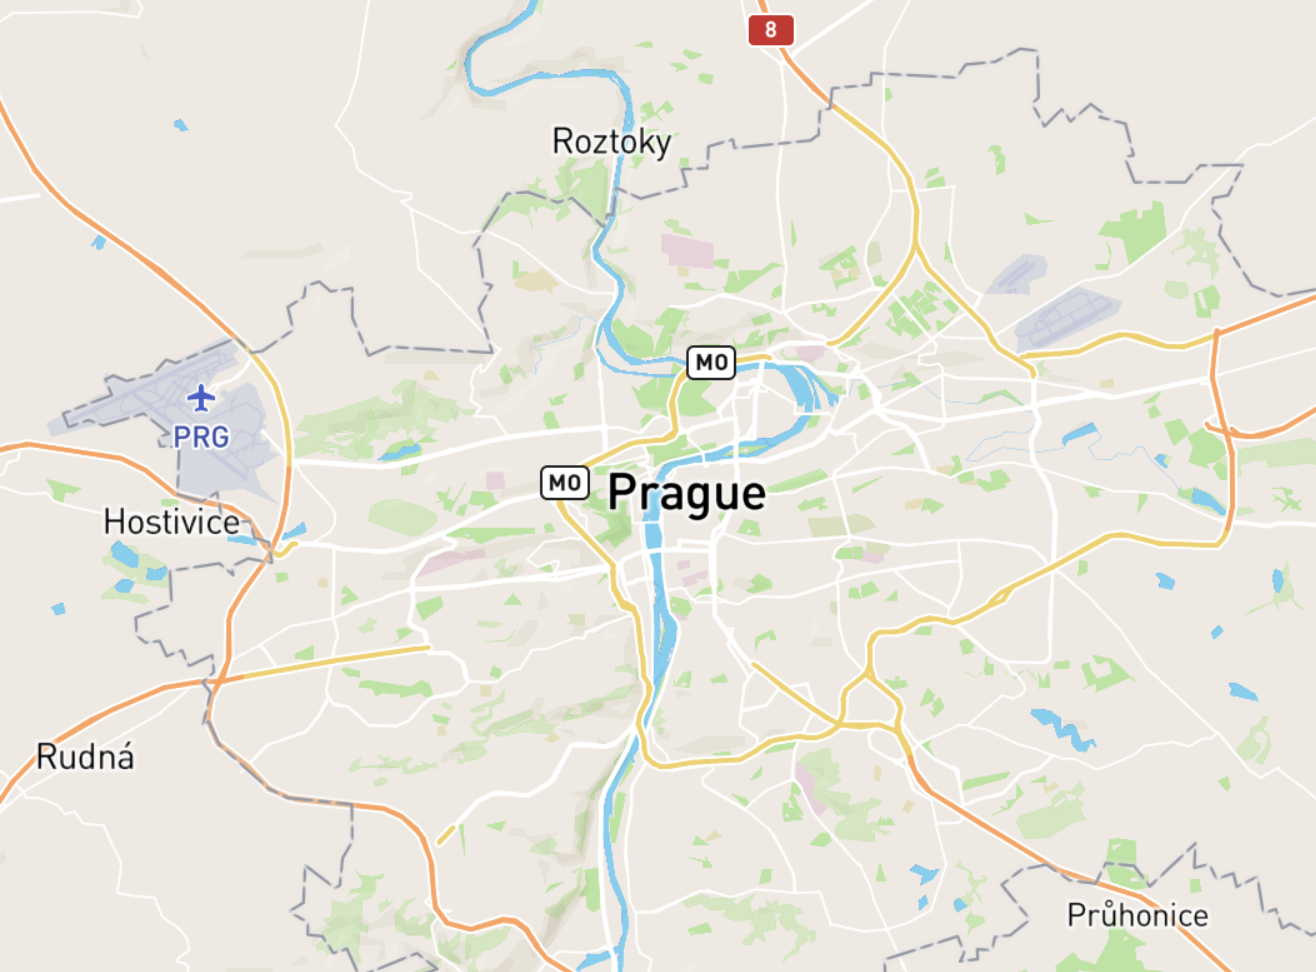
\includegraphics[width=0.5\linewidth]{../img/mapa_mapbox.png}
  \caption{Mapbox Mapa, použitý styl mapy: streets-v11}
  \label{fig:mapbox_mapa}
\end{figure}

Zobrazení jednotlivých spojů bude pomocí bodů v mapě a to konkrétně baravným kruhem s číslem linky, vybrané vozidla se rozliší jinou barvou a velikostí kruhu. Návrh reprezentace vozidel v mapě je zobrazen na obrázku \ref{dve_vozidla}.

\bigbreak

Pro zvolené vozidlo se vykreslí celá jeho trasa včetně všech zastávek. Trasa je reprezentována lomenou čarou a zastávky jako špendlíky v mapě, po přejetí symbolu zastávky se zobrazí i její název. Za zvoleným vozidlem je zobrazena i historie jeho jízdy za uplynulých několik minut, to pomocí barevné lomené čáry, tvořící ocas zvoleného vozidla. Rovněž k povšimnutí na obrázku \ref{dve_vozidla}.

\begin{figure}
	\centering
  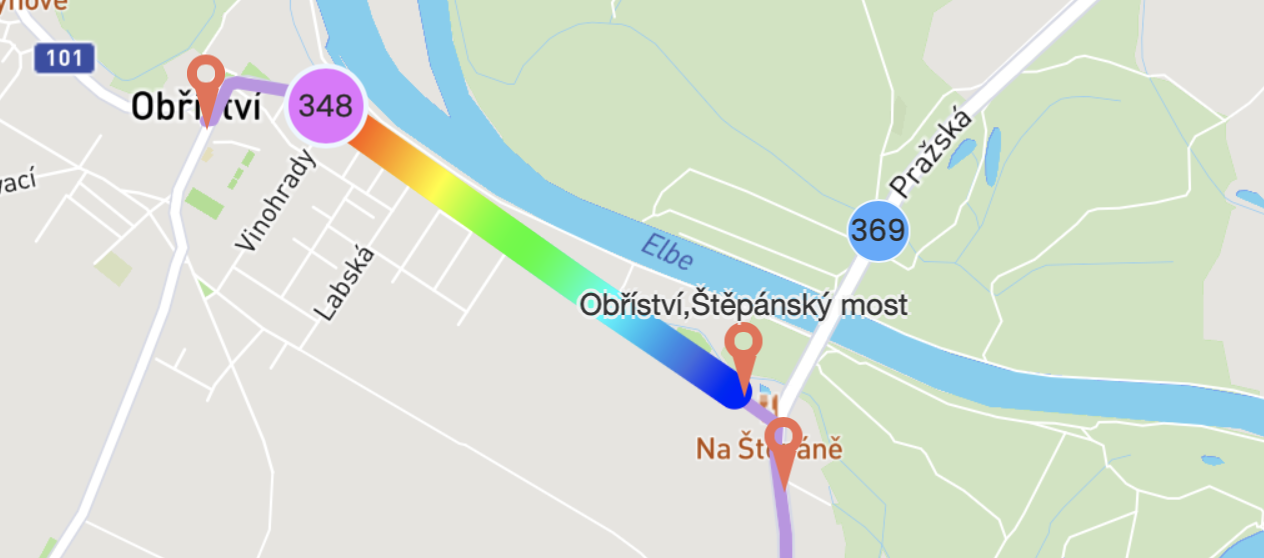
\includegraphics[width=0.5\linewidth]{../img/dve_vozidla.png}
  \caption{Design zobrazení elementů v mapě, linka je 348 je vybrána}
  \label{fig:dve_vozidla}
\end{figure}

Další infomace o spoji, nebo zastávce se zobrazí v tabulce, která z části překryje mapu. Tato tabulka bude obsahovat informace o zvoleném vozidle, konkrétně konečnou stanici, jeho zpoždění a celý jízdní řád. Respektivě infomace o zvolené zastávce a to název zastávky a všechny spoje, které zvolenou zastávkou budou projíždět včetně jejich pravidelného odjezdu a aktuálního zpoždění. Po kliknutí na zastávku se tedy zobrazí její odjedová tabule.
